\section{Porównanie z~wersją prototypową}

W celu porównania działania implementacji w środowisku \textrm{MATLAB} a tej w
\textit{C++}, przefiltrowany został przykładowy sygnał (MIT-BIH 100 próbki
1-250) przy użyciu obu implementacji. Na rysynkach \ref{rys:comp_d1} oraz
\ref{rys:comp_d2} przedstawiono przykładowe wyniki filtracji sygnału EKG,
odpowiednio dla usuniętego 1 i 2-óch IMF-ów.

\begin{figure}[!htb]
    \begin{center}
        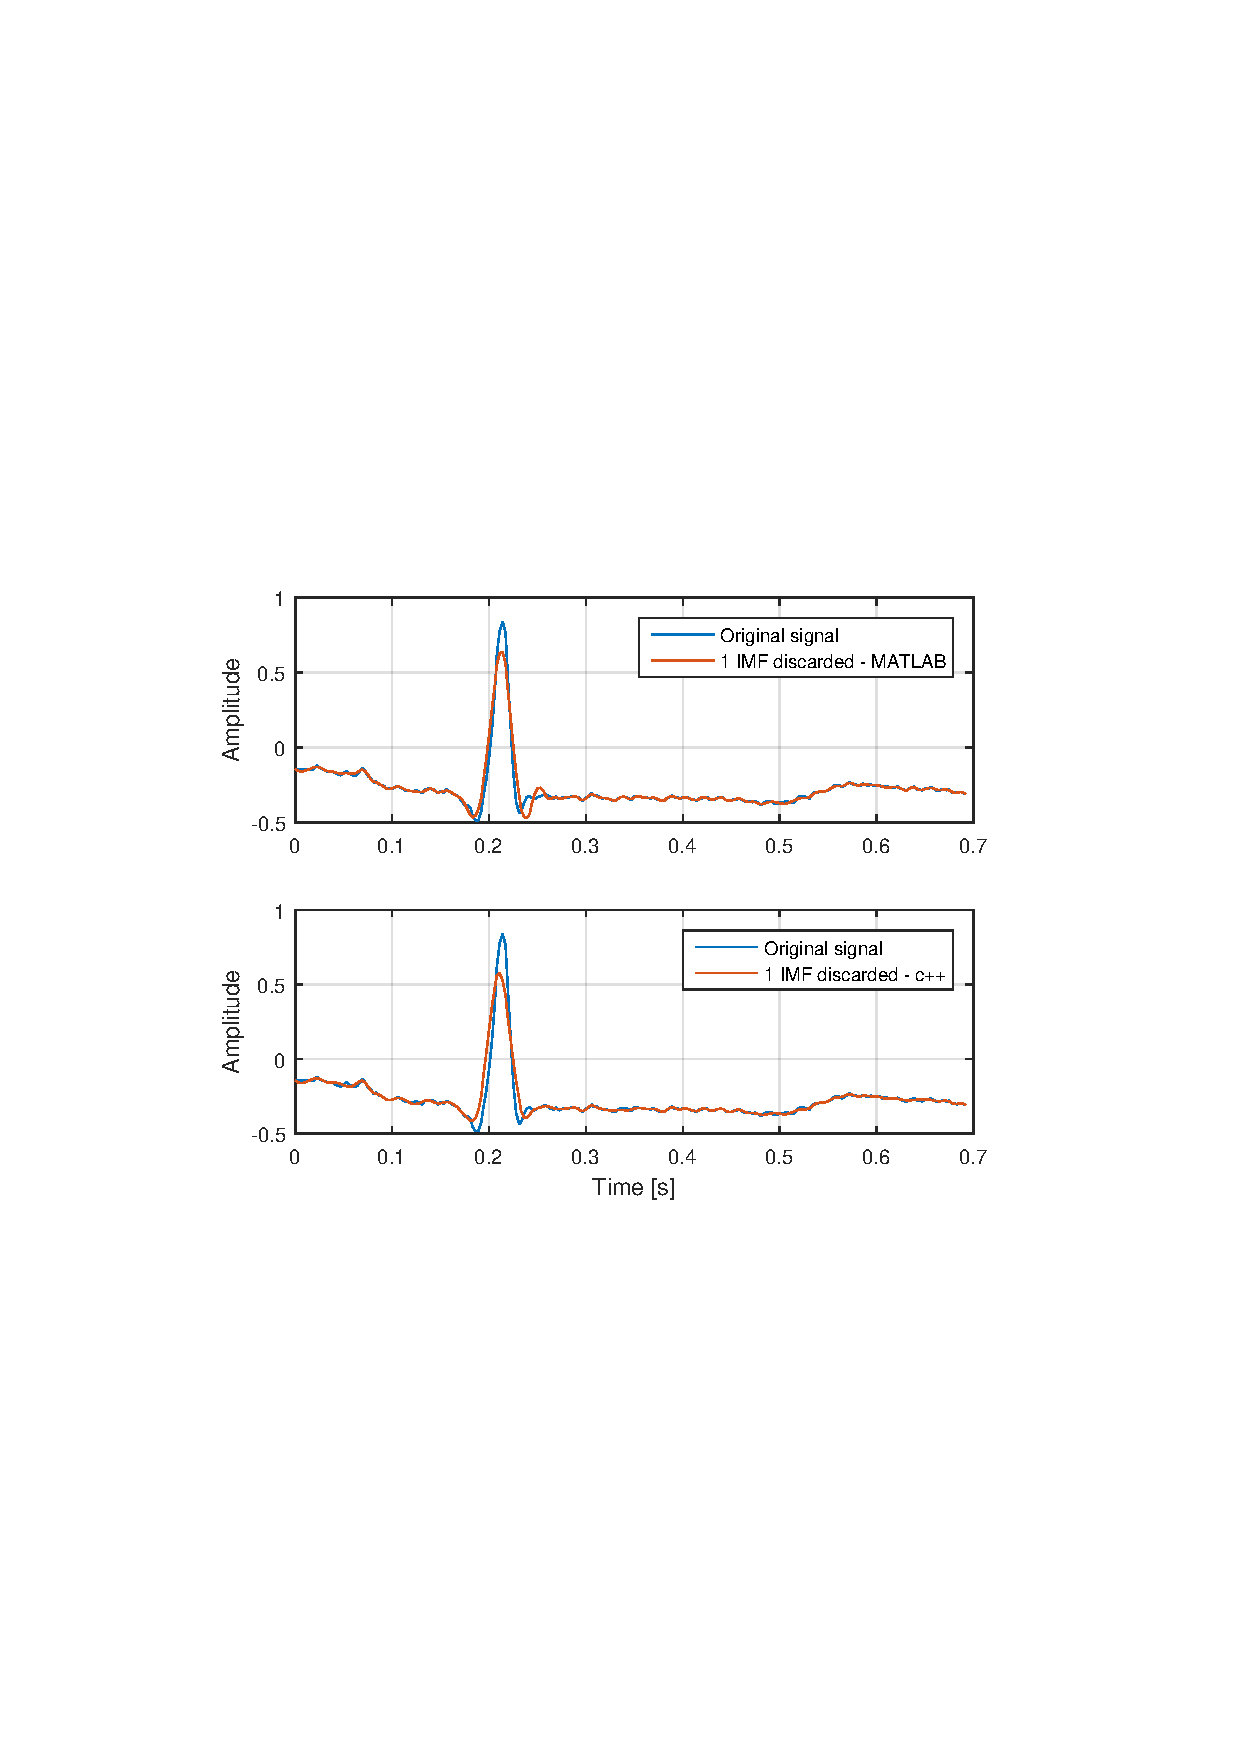
\includegraphics[width=14cm,trim=4cm 9cm 4cm 9cm,clip]
        {../img/mat_cpp_domp_d1.pdf}
    \end{center}
    \caption{Porównanie działania filtracji implementacji \textrm{MATLAB} i
    \textit{C++} przy odrzuceniu 1 IMF-a}
    \label{rys:comp_d1}
\end{figure}

Gołym okiem widać różnice sygnałów przefiltrowanych dwoma implementacjami, zatem
zostały poddane one głębszej analizie.

W jej wyniku odnaleziono przyczynę różnic
wyników w badanych implementacjach. Są one spowodowane przez inne wyniki
wyznaczania funkcji sklejanych w pakietach \textrm{MATLAB} i \textit{Eigen}.
Przykładowe porównanie na przykładzie górnej obwiedni w pierwszej iteracji
algorytmu \textit{emd}, dla sygnału użytego przy porównaniach, znajduje się na
rysunku \ref{rys:comp_spline}.

\newpage

\begin{figure}[!htb]
    \begin{center}
        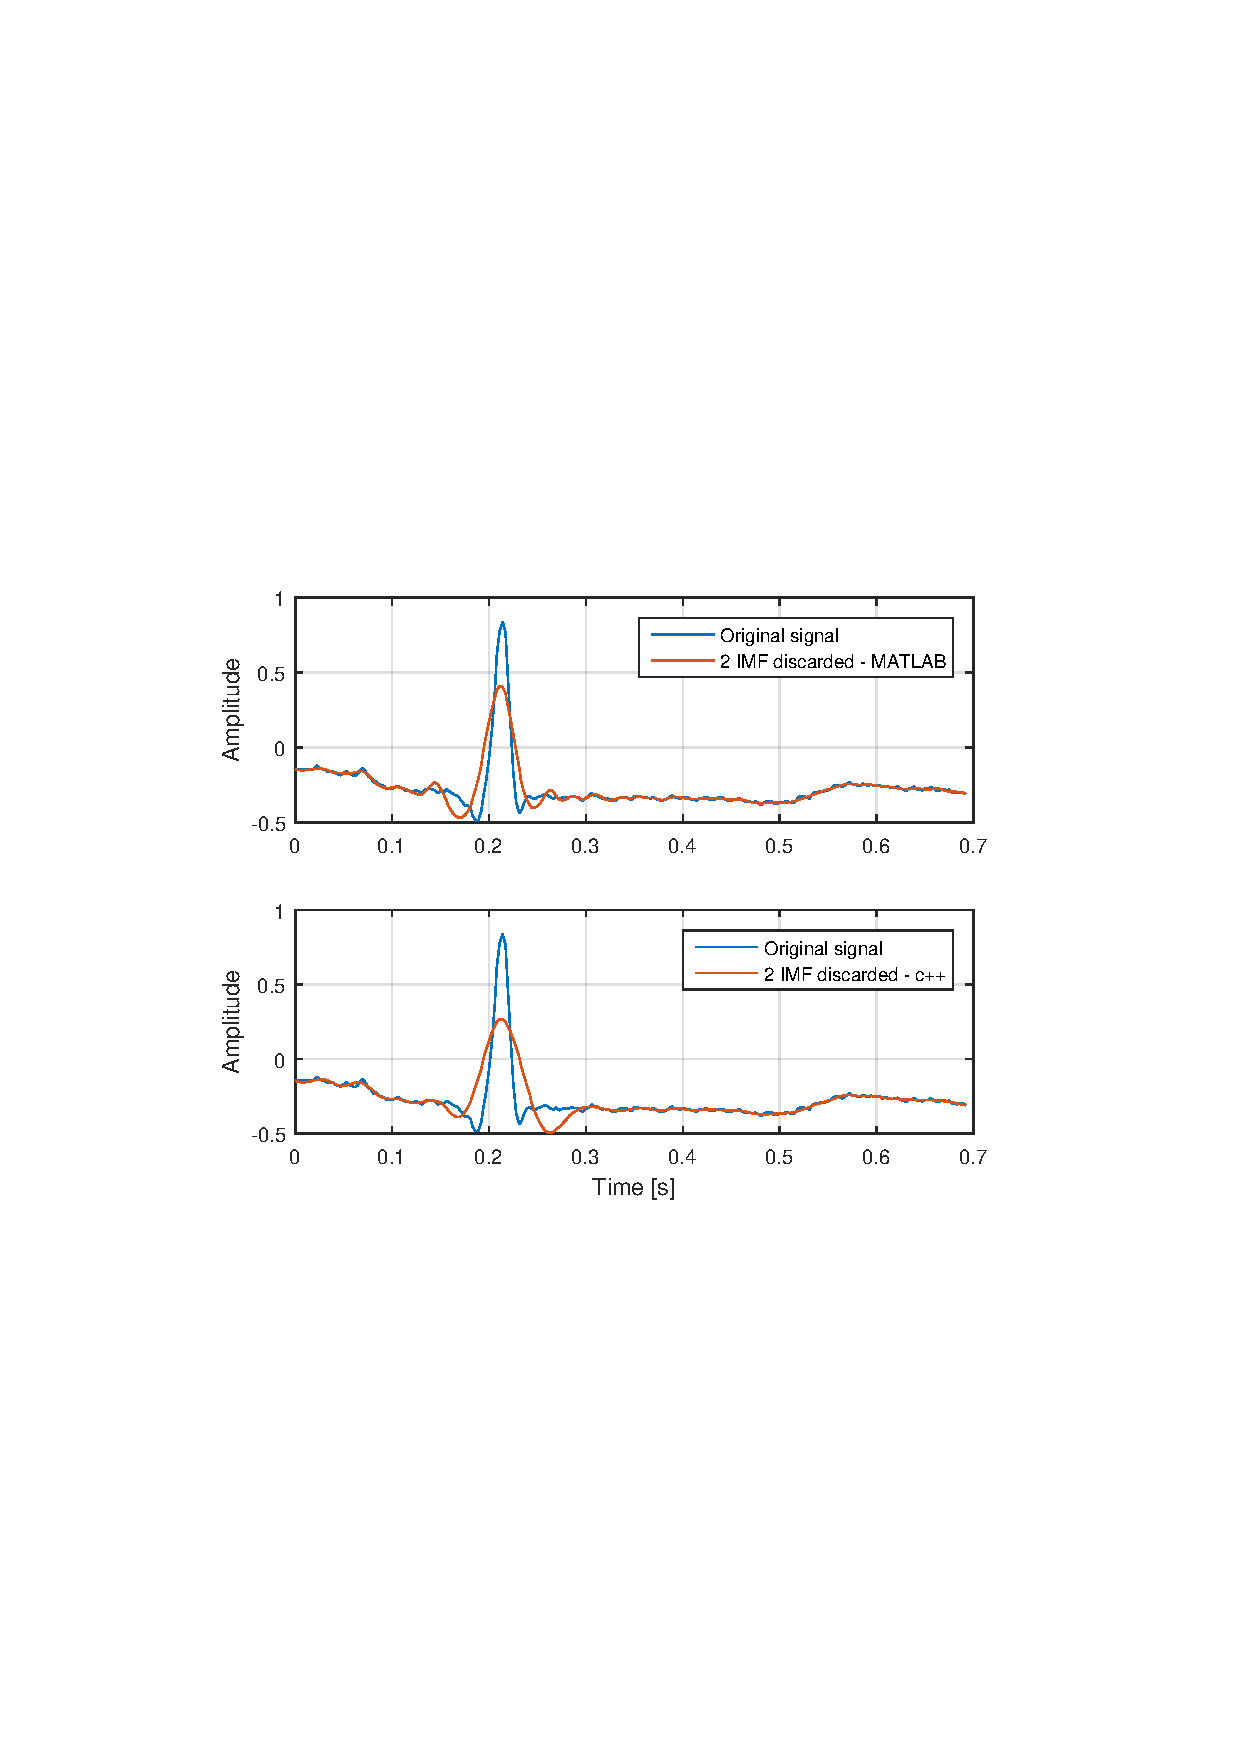
\includegraphics[width=13cm,trim=4cm 9.5cm 4cm 10cm,clip]
        {../img/mat_cpp_domp_d2.pdf}
    \end{center}
    \caption{Porównanie działania filtracji implementacji \textrm{MATLAB} i
    \textit{C++} przy odrzuceniu 2 IMF-ów}
    \label{rys:comp_d2}
\end{figure}

\begin{figure}[!htb]
    \begin{center}
        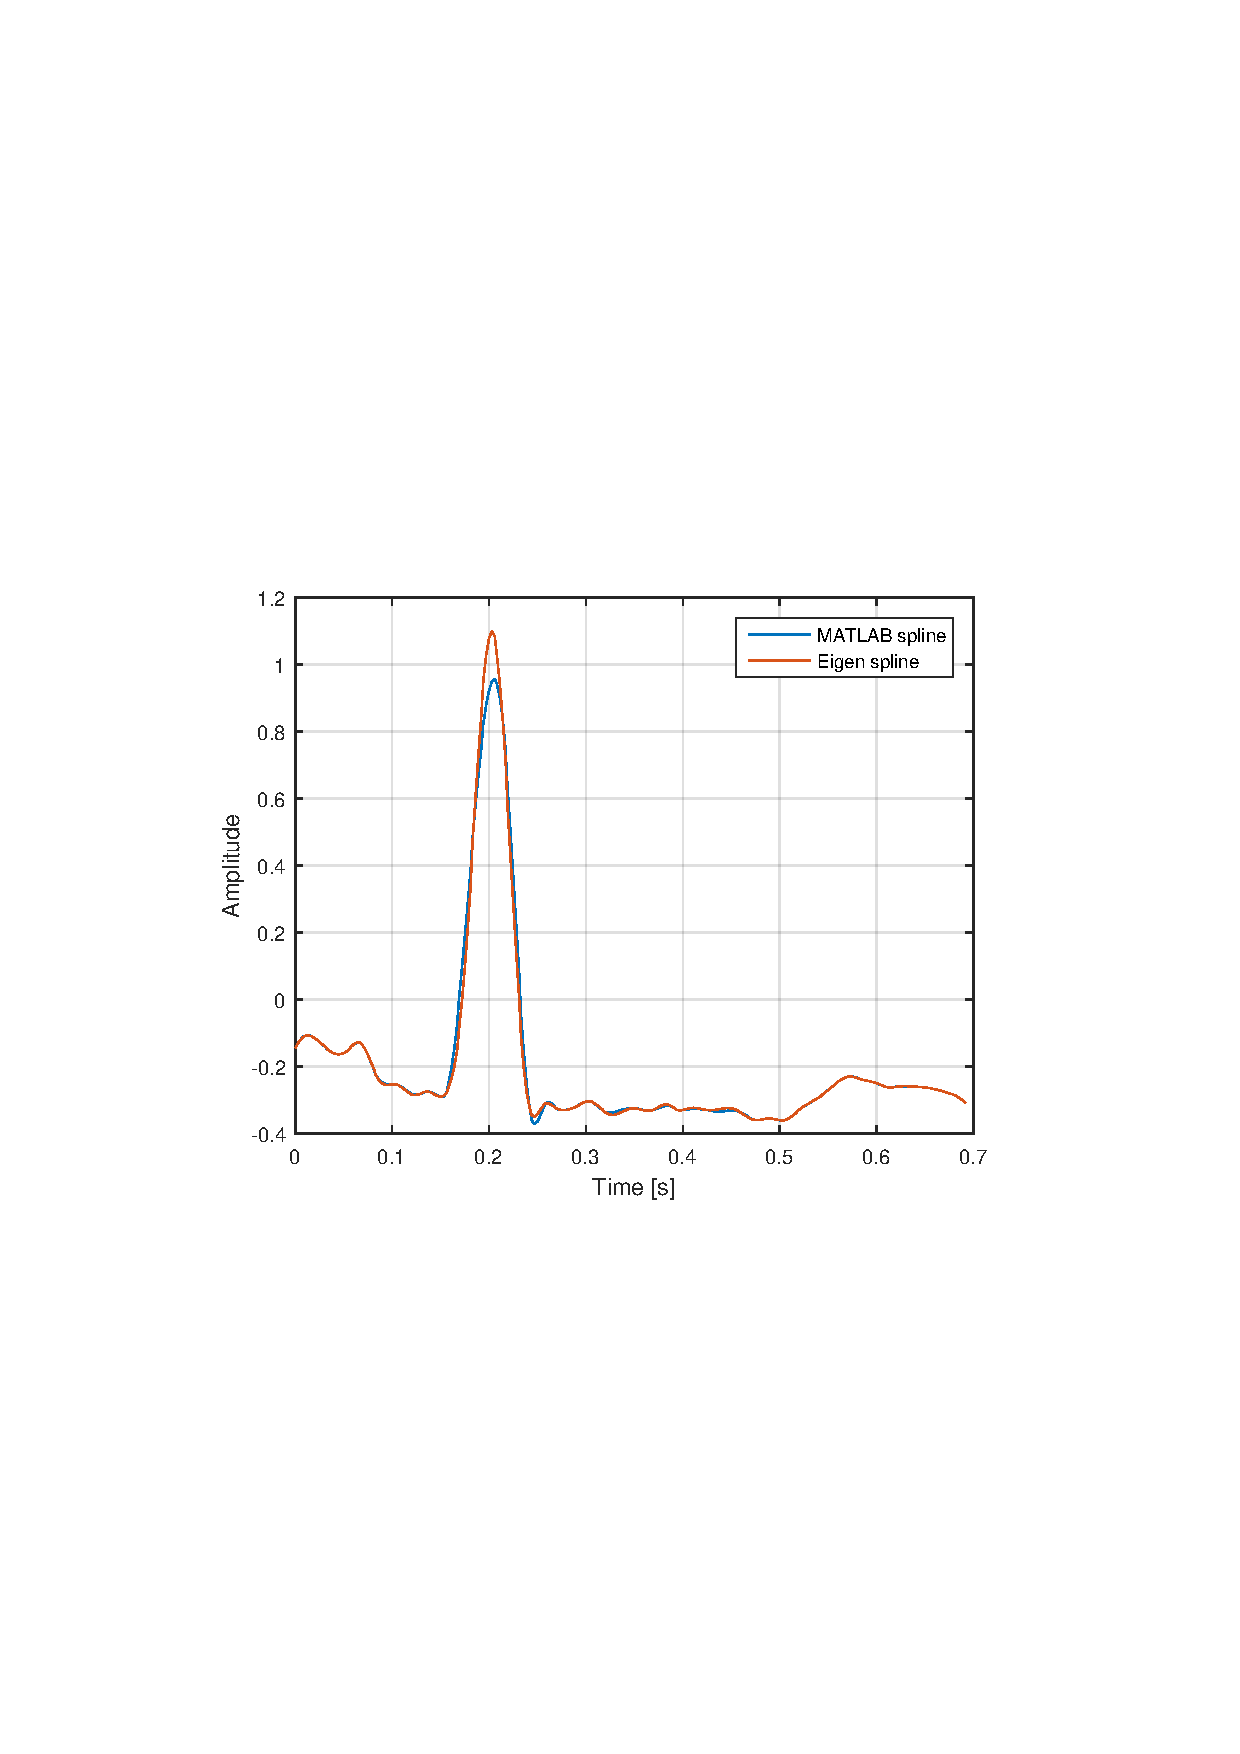
\includegraphics[width=13cm,trim=4cm 9.5cm 4cm 10cm,clip]
        {../img/spline_comp.pdf}
    \end{center}
    \caption{Porównanie implementacji spline-ów pakietów \textit{Eigen} oraz
    \textrm{MATLAB}}
    \label{rys:comp_spline}
\end{figure}
